\documentclass{article}

\usepackage{iclr2026_conference,times}
\usepackage{hyperref}
\usepackage{url}
\usepackage{booktabs}
\usepackage{graphicx}
\usepackage{amsmath}
\usepackage{microtype}

\title{Mood-Based Music Recommendation via\\
Valence--Arousal Classification on the DEAM Dataset}

\author{Anonymous}

\iclrfinalcopy
\begin{document}
\lhead{}

\maketitle

%
\begin{abstract}
%
We present a mood-based music recommendation prototype that maps songs to a
six-class emotional taxonomy derived from Russell's circumplex model of affect,
using the two continuous dimensions of valence (negative--positive) and arousal
(calm--energetic).
A classifier is trained on the DEAM dataset---1{,}802 songs with human
valence/arousal annotations and pre-extracted openSMILE acoustic
features---and evaluated against a random baseline of 16.7\% for six equally
likely classes.
We compare Logistic Regression, Random Forest, SVM with an RBF kernel, and
Gradient Boosting, finding that SVM achieves the best macro F1 of 0.363
and Random Forest the best accuracy at 42.1\%, both more than doubling the
random baseline.
An accompanying command-line prototype classifies new songs using a
lightweight librosa-based arousal/valence proxy and retrieves mood-matched
tracks from a curated catalog.
We additionally characterize a cross-domain feature gap between academic
openSMILE features and deployment-time librosa features, and discuss its
implications for real-world Music Emotion Recognition (MER) systems.
\end{abstract}

%
\section{Introduction}
%

Music streaming platforms serve hundreds of millions of users, yet mood-based
discovery remains a largely unsolved human--computer interaction problem.
Users frequently seek music to match or regulate an emotional state---studying,
exercising, grieving, celebrating---but keyword search and collaborative
filtering offer only coarse proxies for emotional intent.
A system that can automatically predict the emotional character of a song
from its audio content and serve recommendations accordingly would represent
a meaningful improvement in user experience.

The core technical challenge is \emph{Music Emotion Recognition} (MER): given
raw audio or its acoustic features, predict the emotional category a listener
would assign to the song.
This is hard for two reasons.
First, emotion perception is subjective and culturally variable.
Second, the acoustic correlates of emotion are high-dimensional and
non-linear---simple heuristics (e.g., fast tempo $\Rightarrow$ energetic) fail
to capture the full picture.

We address this challenge by framing it as a supervised classification problem
grounded in a principled psychological model.
Specifically, we adopt Russell's \citeyearpar{russell1980circumplex}
circumplex model of affect, which represents emotions as points in a continuous
two-dimensional space spanned by \emph{valence} (how positive or negative the
emotion is) and \emph{arousal} (how activating or calming it is).
By discretising this space into six named mood regions (Figure~\ref{fig:moodspace}),
we obtain a taxonomy that is both psychologically grounded and practically
interpretable by users.

The contributions of this work are:
\begin{enumerate}
    \item A six-class valence--arousal mood taxonomy applied to the DEAM
          benchmark, with a systematic comparison of four classifiers.
    \item An end-to-end recommendation prototype that covers data ingestion,
          model training, catalog labeling, and user-facing retrieval.
    \item An empirical characterisation of the cross-domain feature gap between
          openSMILE-extracted training features and librosa-extracted deployment
          features, with discussion of its implications for MER system design.
\end{enumerate}

%
\section{Related Work}
%

\paragraph{Dimensional models of music emotion.}
The idea that music emotion can be represented as a point in a continuous
two-dimensional space traces back to \citet{russell1980circumplex}, whose
circumplex model organises emotions around the axes of valence and arousal.
\citet{thayer1989biopsychology} applied a similar two-dimensional framework
specifically to music, and subsequent MER work has largely adopted these axes
as the prediction targets \citep{yang2012machine}.

\paragraph{Datasets for MER.}
Early MER datasets relied on genre proxies or single-label categorical
annotations.
\citet{eerola2011comparison} provided an extensive comparison of annotation
schemes and showed that dimensional (valence/arousal) ratings correlate more
reliably across raters than categorical labels.
The DEAM dataset \citep{aljanaki2017developing} addresses this by collecting
continuous per-second valence/arousal ratings from crowdsourced annotators
across 1{,}802 songs, making it the largest publicly available benchmark for
dimensional MER and the dataset used in this work.

\paragraph{Acoustic features for MER.}
\citet{eyben2010opensmile} introduced openSMILE, a real-time feature extractor
that computes a standardised set of low-level acoustic descriptors (MFCCs,
pitch, energy, zero-crossing rate, and spectral shape statistics) widely used
in speech and music affective computing challenges.
\citet{mcfee2015librosa} subsequently released librosa, a Python library
providing overlapping functionality with a simpler API, which has become the
standard tool for rapid MER prototyping.

\paragraph{Classification approaches.}
\citet{yang2012machine} survey early MER systems and find that SVMs with
radial basis function kernels are consistently competitive.
More recent work has explored deep learning \citep{pons2017timbre}, but on
smaller datasets (under 1{,}000 songs) handcrafted acoustic features paired
with SVMs or Random Forests remain strong baselines \citep{eerola2011comparison}.
Our work follows this tradition while extending from the standard two- or
three-class formulation to a more user-interpretable six-class taxonomy.

\paragraph{Music recommendation.}
Most commercial recommendation systems rely on collaborative filtering and
do not directly model audio content \citep{schedl2018current}.
Content-based approaches that do use audio features tend to target genre or
tempo rather than emotion \citep{tzanetakis2002musical}.
Our prototype fills this gap by using a classifier trained on human emotional
annotations to drive content-based retrieval.

%
\section{Methodology}
%

\subsection{Mood Taxonomy}

We define six mood classes by partitioning the continuous valence--arousal
plane at data-driven thresholds.
Specifically, we compute the 33rd and 66th percentiles of the DEAM arousal
and valence distributions and use these to divide the plane into a $3 \times 2$
grid (Figure~\ref{fig:moodspace}).
The resulting classes---\textit{blue}, \textit{calm}, \textit{focus},
\textit{love}, \textit{energetic}, and \textit{feel good}---span the full
affective space and carry intuitive user-facing labels.
Using data-driven percentile thresholds rather than fixed boundaries ensures
balanced class sizes, which stabilises classifier training.

\begin{figure}[h]
    \centering
    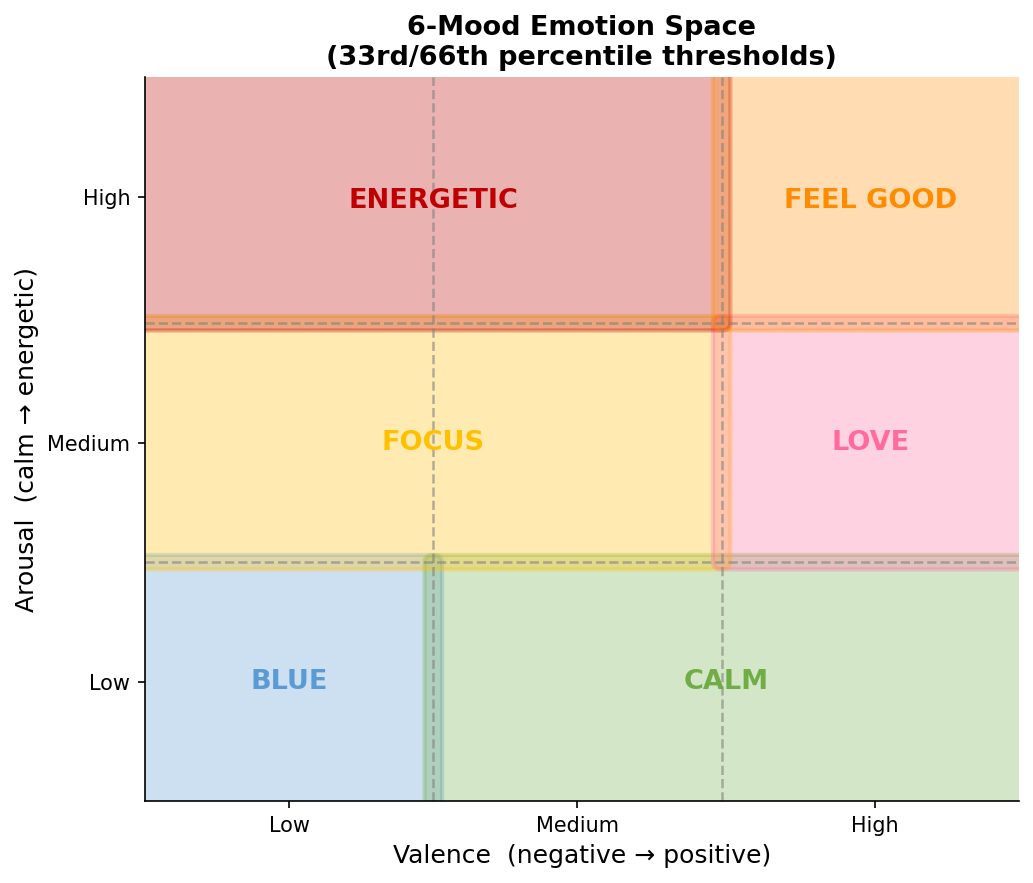
\includegraphics[width=0.62\linewidth]{figures/slide2_mood_space.png}
    \caption{Six-class mood taxonomy derived from the DEAM valence--arousal
             distribution. Dashed lines show the 33rd/66th percentile
             thresholds on each axis.}
    \label{fig:moodspace}
\end{figure}

\subsection{Dataset and Features}

We use the DEAM dataset \citep{aljanaki2017developing}, which provides
song-level mean valence and arousal ratings for 1{,}802 45-second clips
sourced from the Free Music Archive.
Pre-extracted openSMILE features \citep{eyben2010opensmile} are provided with
the dataset; each song is represented by a per-frame CSV of IS09-configuration
low-level descriptors (LLDs) including RMS energy, zero-crossing rate,
fundamental frequency, voicing probability, MFCCs 1--12, and their delta
coefficients, as well as spectral shape statistics (centroid, flux, rolloff,
entropy, harmonicity).
Following standard practice, we average all per-frame values to obtain a
single song-level feature vector.
After merging features with annotations, 1{,}802 songs are available; we use
an 80/20 stratified train/test split ($n_\text{train}=1{,}441$,
$n_\text{test}=361$).

\subsection{Classifier Comparison}

We train four classifiers, all with \texttt{StandardScaler} normalisation
applied inside a scikit-learn \texttt{Pipeline}:

\begin{itemize}
    \item \textbf{Logistic Regression} (\texttt{max\_iter=4000},
          \texttt{class\_weight=balanced})
    \item \textbf{Random Forest} (300 trees, \texttt{class\_weight=balanced},
          \texttt{random\_state=0})
    \item \textbf{SVM with RBF kernel} (\texttt{class\_weight=balanced},
          \texttt{probability=True}, \texttt{random\_state=0})
    \item \textbf{Gradient Boosting} (300 estimators,
          \texttt{random\_state=0})
\end{itemize}

The \texttt{class\_weight=balanced} setting compensates for slight class
imbalance introduced by the percentile-based labeling.

\subsection{Recommendation Prototype}

The recommendation prototype consists of two offline stages and one
online stage.

\textbf{Catalog building (offline).}
A curated list of 48 well-known songs spanning all six moods is processed
by \texttt{build\_catalog.py}.
For each song, a 30-second audio clip is located and downloaded via
\texttt{yt-dlp}.
Acoustic features are extracted using librosa \citep{mcfee2015librosa}:
tempo, RMS energy, zero-crossing rate, spectral centroid, spectral rolloff,
12 MFCCs with their standard deviations, 12 chroma coefficients, and 7
spectral contrast bands.
Arousal and valence proxies are derived from these features using weighted
combinations: arousal is estimated from RMS energy (weight 0.35), tempo
(0.30), zero-crossing rate (0.20), and spectral centroid (0.15); valence is
estimated from a Krumhansl--Schmuckler key-profile score
\citep{krumhansl1990cognitive} indicating major/minor mode (weight 0.65)
and low-band spectral contrast (0.35).
Each song is then assigned a mood class using the same six-region taxonomy
as the DEAM experiment.

\textbf{Cross-domain gap (offline analysis).}
We investigated whether the DEAM-trained SVM could be applied directly to
catalog songs using features extracted by the Python \texttt{opensmile}
package \citep{eyben2010opensmile}.
Despite using the same nominal IS09 configuration, we found a systematic
distributional shift: MFCC\,1 means differ by approximately 31 units
($\mu_\text{DEAM}=24.6$ vs.\ $\mu_\text{catalog}=-6.7$), and RMS energy
means differ by a factor of six ($0.109$ vs.\ $0.017$).
This shift arises from differences between the original openSMILE
command-line tool used for DEAM preprocessing and the Python package's
internal audio pipeline.
As a result, direct cross-domain inference collapses all catalog songs into
a single class; we therefore retain the librosa proxy for deployment and
discuss domain adaptation as future work (Section~\ref{sec:conclusion}).

\textbf{Retrieval (online).}
\texttt{recommend.py} accepts a target mood and returns the top-$k$ songs
from the catalog matching that mood, ordered by descending mean RMS energy
as a secondary signal of intensity within the class.

%
\section{Experimental Results}
%

\subsection{Classifier Comparison on DEAM}

Table~\ref{tab:results} reports accuracy and macro-averaged F1 for all four
models on the held-out test set.
The SVM with an RBF kernel achieves the highest macro F1 (0.363) while
Logistic Regression is a close second (0.361).
All models substantially outperform the random baseline of 16.7\%
(six equally likely classes), confirming that acoustic features carry
meaningful mood signal.

\begin{table}[h]
\centering
\caption{Six-class mood classification results on the DEAM test set
         ($n=361$). Best macro F1 is \textbf{bolded}.
         Random baseline accuracy and macro F1 are both 0.167.}
\label{tab:results}
\begin{tabular}{lcc}
\toprule
\textbf{Model} & \textbf{Accuracy} & \textbf{Macro F1} \\
\midrule
Logistic Regression & 0.391 & 0.361 \\
Random Forest       & 0.421 & 0.341 \\
SVM (RBF)           & 0.385 & \textbf{0.363} \\
Gradient Boosting   & 0.413 & 0.348 \\
\midrule
Random baseline     & 0.167 & 0.167 \\
\bottomrule
\end{tabular}
\end{table}

Figure~\ref{fig:comparison} contextualises these results against the CP1
baseline: a Logistic Regression classifier on a simpler \emph{three-class}
arousal task (calm / medium / energetic) achieved 58\% accuracy and macro
F1 of 0.576.
The reduction in performance when moving to six classes is expected---the
problem becomes strictly harder---but the absolute improvement over the
six-class random baseline (0.363 vs.\ 0.167) is proportionally larger.

\begin{figure}[h]
    \centering
    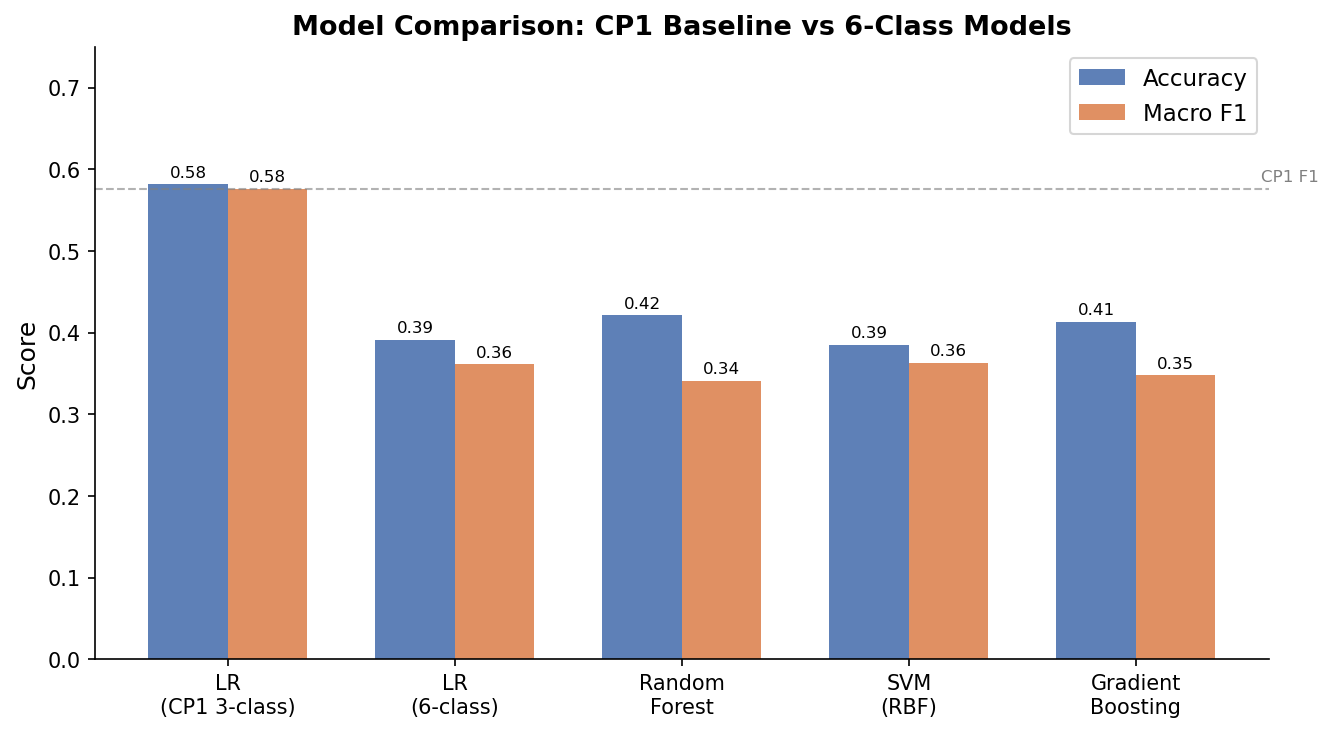
\includegraphics[width=0.85\linewidth]{figures/slide7_model_comparison.png}
    \caption{Model comparison. The leftmost bar is the CP1 3-class baseline
             (Logistic Regression on arousal only). Remaining bars show
             6-class performance across all models evaluated in this work.}
    \label{fig:comparison}
\end{figure}

\subsection{Per-Class Analysis}

Examining the SVM's per-class F1 scores reveals a consistent pattern aligned
with the structure of the mood space.
The \textit{blue} class (low arousal, low valence) achieves the highest F1
at 0.613, benefiting from its corner position in the valence--arousal plane
which gives it the most distinctive acoustic signature.
The \textit{feel good} class (high arousal, high valence) follows at 0.420.
Mid-plane classes---\textit{focus} (0.283) and \textit{love} (0.214)---are
hardest to classify, as they occupy the centre of the arousal--valence space
where boundaries between adjacent classes are most ambiguous.
This pattern is consistent with findings in \citet{eerola2011comparison},
who note that extreme-valence categories are generally more reliably annotated
and classified than intermediate ones.

\subsection{Recommendation Prototype Results}

The catalog contains 48 songs distributed across six mood classes:
energetic (14), calm (11), focus (10), love (6), blue (5), and feel good (2).
The \textit{feel good} class is underrepresented because the librosa valence
proxy---which relies on a Krumhansl--Schmuckler key profile---produces a
narrow valence range across most songs, clustering them near the median and
leaving few above the 66th percentile threshold.
This suggests that key-profile-based valence estimation is an insufficient
proxy on its own, consistent with \citet{yang2012machine} who find valence
harder to predict from audio than arousal.

Example recommendations for \texttt{--mood calm --k 5}: \textit{So What}
(Miles Davis), \textit{Come Away with Me} (Norah Jones), \textit{Music for
Airports} (Brian Eno), \textit{Death With Dignity} (Sufjan Stevens), and
\textit{Your Hand in Mine} (Explosions in the Sky).
These are qualitatively appropriate calm recommendations, suggesting the
librosa proxy is effective for the arousal axis despite its valence limitations.

%
\section{Conclusion}
\label{sec:conclusion}
%

We presented a mood-based music recommendation prototype grounded in a
psychologically motivated six-class valence--arousal taxonomy.
Our classifier comparison on the DEAM benchmark shows that an SVM with an
RBF kernel achieves the best macro F1 of 0.363 at 38.5\% accuracy,
more than doubling the random baseline of 16.7\%.
The recommendation prototype demonstrates that mood-conditioned retrieval
from an acoustically labeled catalog is feasible with off-the-shelf tools.

A central finding of this work is the \textbf{cross-domain feature gap}
between academic feature sets (openSMILE command-line) and deployment feature
sets (opensmile Python package / librosa).
Even when nominally extracting the same IS09 features, distributional
shifts of up to 31 units in MFCC means and a factor of six in RMS energy
render direct model transfer infeasible.
This gap is underreported in the MER literature, where training and inference
typically share the same feature extraction pipeline.

\paragraph{Future work.}
Three directions would meaningfully strengthen this system.
First, downloading DEAM audio and re-extracting librosa features would close
the domain gap and enable a unified training and inference pipeline.
Second, improving the valence proxy---for example via chord-progression
analysis or pre-trained audio encoders such as MusicGen
\citep{copet2023musicgen}---would address the clustering of songs near the
valence median.
Third, extending the catalog from 48 to thousands of songs (e.g., via the
Spotify or Last.fm APIs) would make the prototype viable for real users.

\paragraph{Code availability.}
All code, the pre-built song catalog, and the trained model are available at
\url{https://github.com/luisdiazgranados/ECE570Project}.

\paragraph{LLM usage.}
Claude (Anthropic) was used as a coding assistant during development of this
project, specifically for debugging and code review. All algorithmic design
decisions, experimental choices, and written content are the authors' own.

%
\bibliography{refs}
\bibliographystyle{iclr2026_conference}
%

\end{document}
